\documentclass{beamer}
\usepackage{xcolor}
\usepackage{mathtools}
\usetheme[titlepagelogo=firenze,% Logo for the first page
		  language=italian,
		  bullet=circle,
		  color=blue,
         ]{TorinoTh}
\usepackage[beamer,customcolors]{hf-tikz}
\definecolor{UniBlue}{RGB}{83,121,170}
\setbeamercolor{block title}{use=structure,fg=white,bg=UniBlue}
\setbeamercolor{block body}{use=structure,fg=black,bg=white}

\newcommand*{\bfrac}[2]{\genfrac{}{}{0pt}{1}{#1}{#2}}

\author{}
\rel{{\normalsize \emph{Visual and Multimedia Recognition}}\\\vspace{0.3cm}Lorenzo Cioni}
\title{\huge Improving WATSS web application with Computer Vision techniques}
\date{}

\begin{document}

\titlepageframe

\begin{tframe}{Introduction}

WATSS, \textbf{Web Annotation Tool for Surveillance Scenarios}, is a web-based annotation tool developed to annotate dataset in surveillance systems.

\vspace{0.3cm}

\textbf{Main goal}: improve WATSS with some \textbf{Computer Vision approaches}, in order to make easy for users to use this tool and make the annotation process more \emph{automatic}

\begin{figure}[h]
\begin{center}
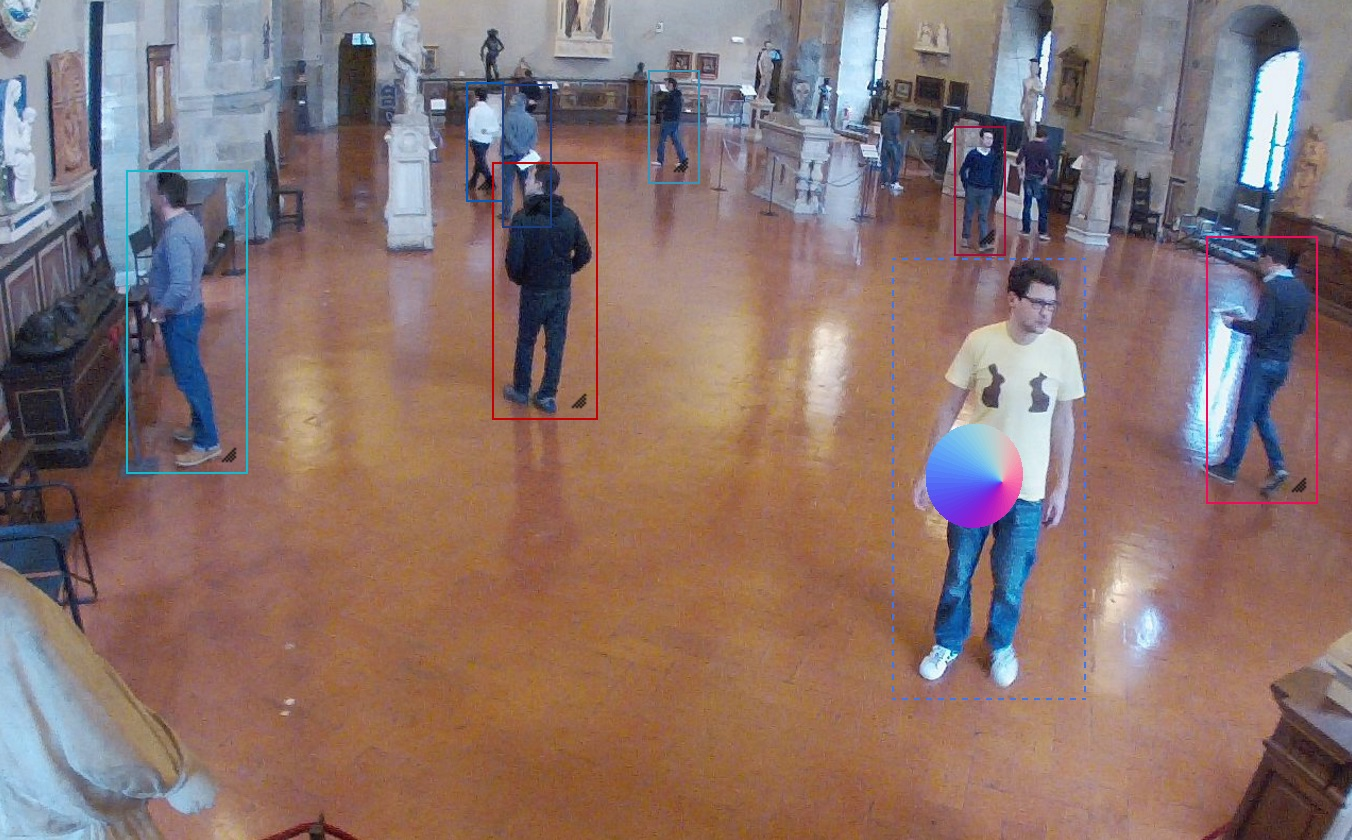
\includegraphics[width=0.4\textwidth]{images/frame.jpg}
\end{center}
\label{fig:mainframe}
\end{figure}

\end{tframe}

\begin{tframe}{Comparative analysis of annotation tools}
\textbf{LabelMe} 
\begin{columns}[t] % align columns
\begin{column}{.5\textwidth}
\begin{itemize}
\item \textbf{Web-based} tool, also for mobile applications
\vspace{0.2cm}
\item Annotate scenes with \textbf{polygonal areas}
\vspace{0.2cm}
\item \textbf{Nested} objects and \textbf{occlusion} annotation
\vspace{0.2cm}
\item \emph{Zoom in} and \emph{out} of the scene
\end{itemize}
\end{column}%
\begin{column}{.3\textwidth}
\begin{figure}[h]
\centering
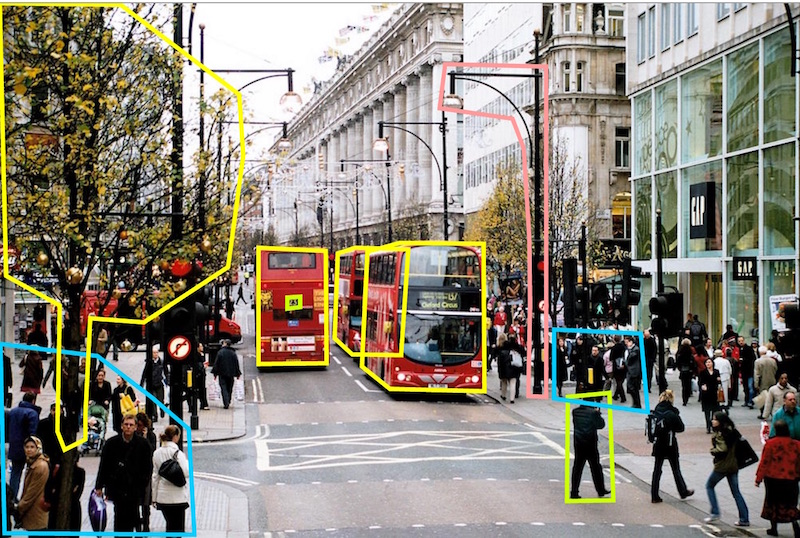
\includegraphics[width=1\textwidth]{images/labelme.jpg}
\end{figure}
\end{column}%
\end{columns}
\end{tframe}


\begin{tframe}{Comparative analysis of annotation tools}
\textbf{ViPER-GT} 
\begin{columns}[t] % align columns
\begin{column}{.5\textwidth}
\begin{itemize}
\item \textbf{Java application} tool
\vspace{0.2cm}
\item Annotate scenes with \textbf{geometrical shapes}
\vspace{0.2cm}
\item \textbf{Timeline} and \textbf{annotation highlighting} on time change
\vspace{0.2cm}
\item Linear \textbf{interpolation} between annotations
\vspace{0.2cm}
\item \emph{Zoom in} and \emph{out} of the scene
\end{itemize}
\end{column}%
\begin{column}{.3\textwidth}
\begin{figure}[h]
\centering
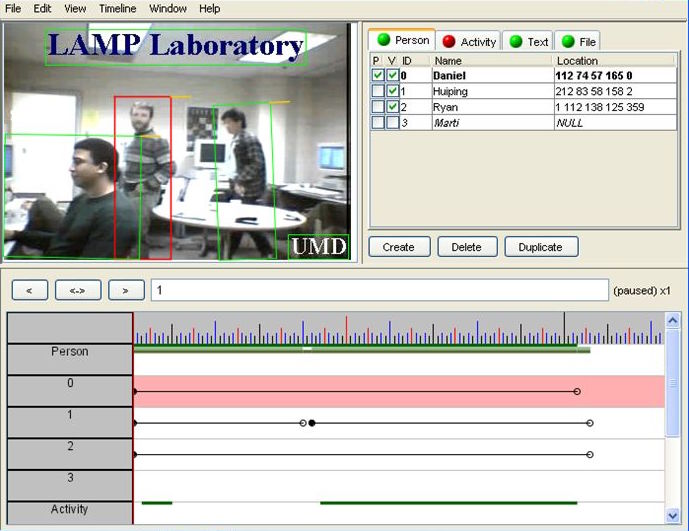
\includegraphics[width=1\textwidth]{images/vipergt.jpg}
\end{figure}
\end{column}%
\end{columns}
\end{tframe}

\begin{tframe}{Comparative analysis of annotation tools}
\textbf{VATIC} 
\begin{columns}[t] % align columns
\begin{column}{.45\textwidth}
\begin{itemize}
\item \textbf{Online} tool
\vspace{0.1cm}
\item Developed for \textbf{object detection}
\vspace{0.1cm}
\item \textbf{Crowd-sourcing} to Amazon's \emph{Mechanical Turk}
\vspace{0.1cm}
\item Multiple \textbf{plugins}: \emph{object tracking}, \emph{sentence annotation}, etc.
\end{itemize}
\end{column}%
\begin{column}{.3\textwidth}
\begin{figure}[h]
\centering
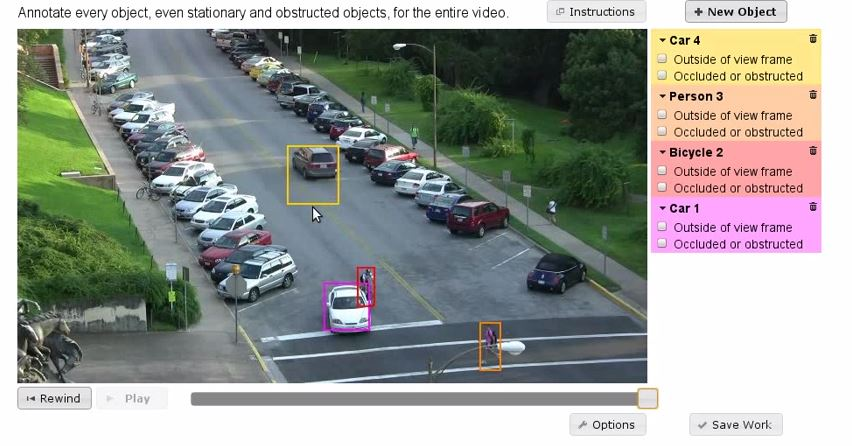
\includegraphics[width=1.2\textwidth]{images/vatic.jpg}
\end{figure}
\end{column}%
\end{columns}
\end{tframe}

\begin{tframe}{Comparative analysis of annotation tools}
\textbf{WATSS} 
\begin{columns}[t] % align columns
\begin{column}{.45\textwidth}
\begin{itemize}
\item \textbf{Web-based} tool
\vspace{0.1cm}
\item Annotation with bounding box
\vspace{0.1cm}
\item \textbf{Occlusion} area
\vspace{0.1cm}
\item Coarse \textbf{gaze} estimation
\vspace{0.1cm}
\item \textbf{Groups} and POI under observation
\vspace{0.1cm}
\item \textbf{Multiple cameras} manager
\end{itemize}
\end{column}%
\begin{column}{.3\textwidth}
\begin{figure}[h]
\centering
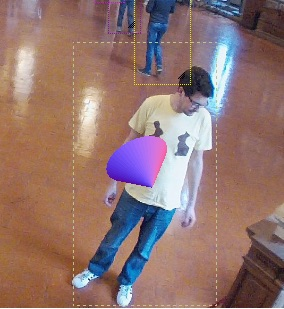
\includegraphics[width=1\textwidth]{images/gaze.jpg}
\end{figure}
\end{column}%
\end{columns}
\end{tframe}


\begin{tframe}{Improvements}
\begin{itemize}
\vspace{0.3cm}
\item \textbf{User interface} renovation
\vspace{0.2cm}
\item Simpler annotation making and editing
\vspace{0.2cm}
\item Video \textbf{timeline} for annotations
\vspace{0.2cm}
\item Annotation automatic \textbf{proposals} generation
\vspace{0.2cm}
\item \textbf{Scene geometry}-based enhancement
\vspace{0.2cm}
\item Easy \textbf{setup} process
\end{itemize}
\end{tframe}

\begin{tframe}{User interface renovation}
The \textbf{old} WATSS user interface
\begin{figure}[h]
\centering
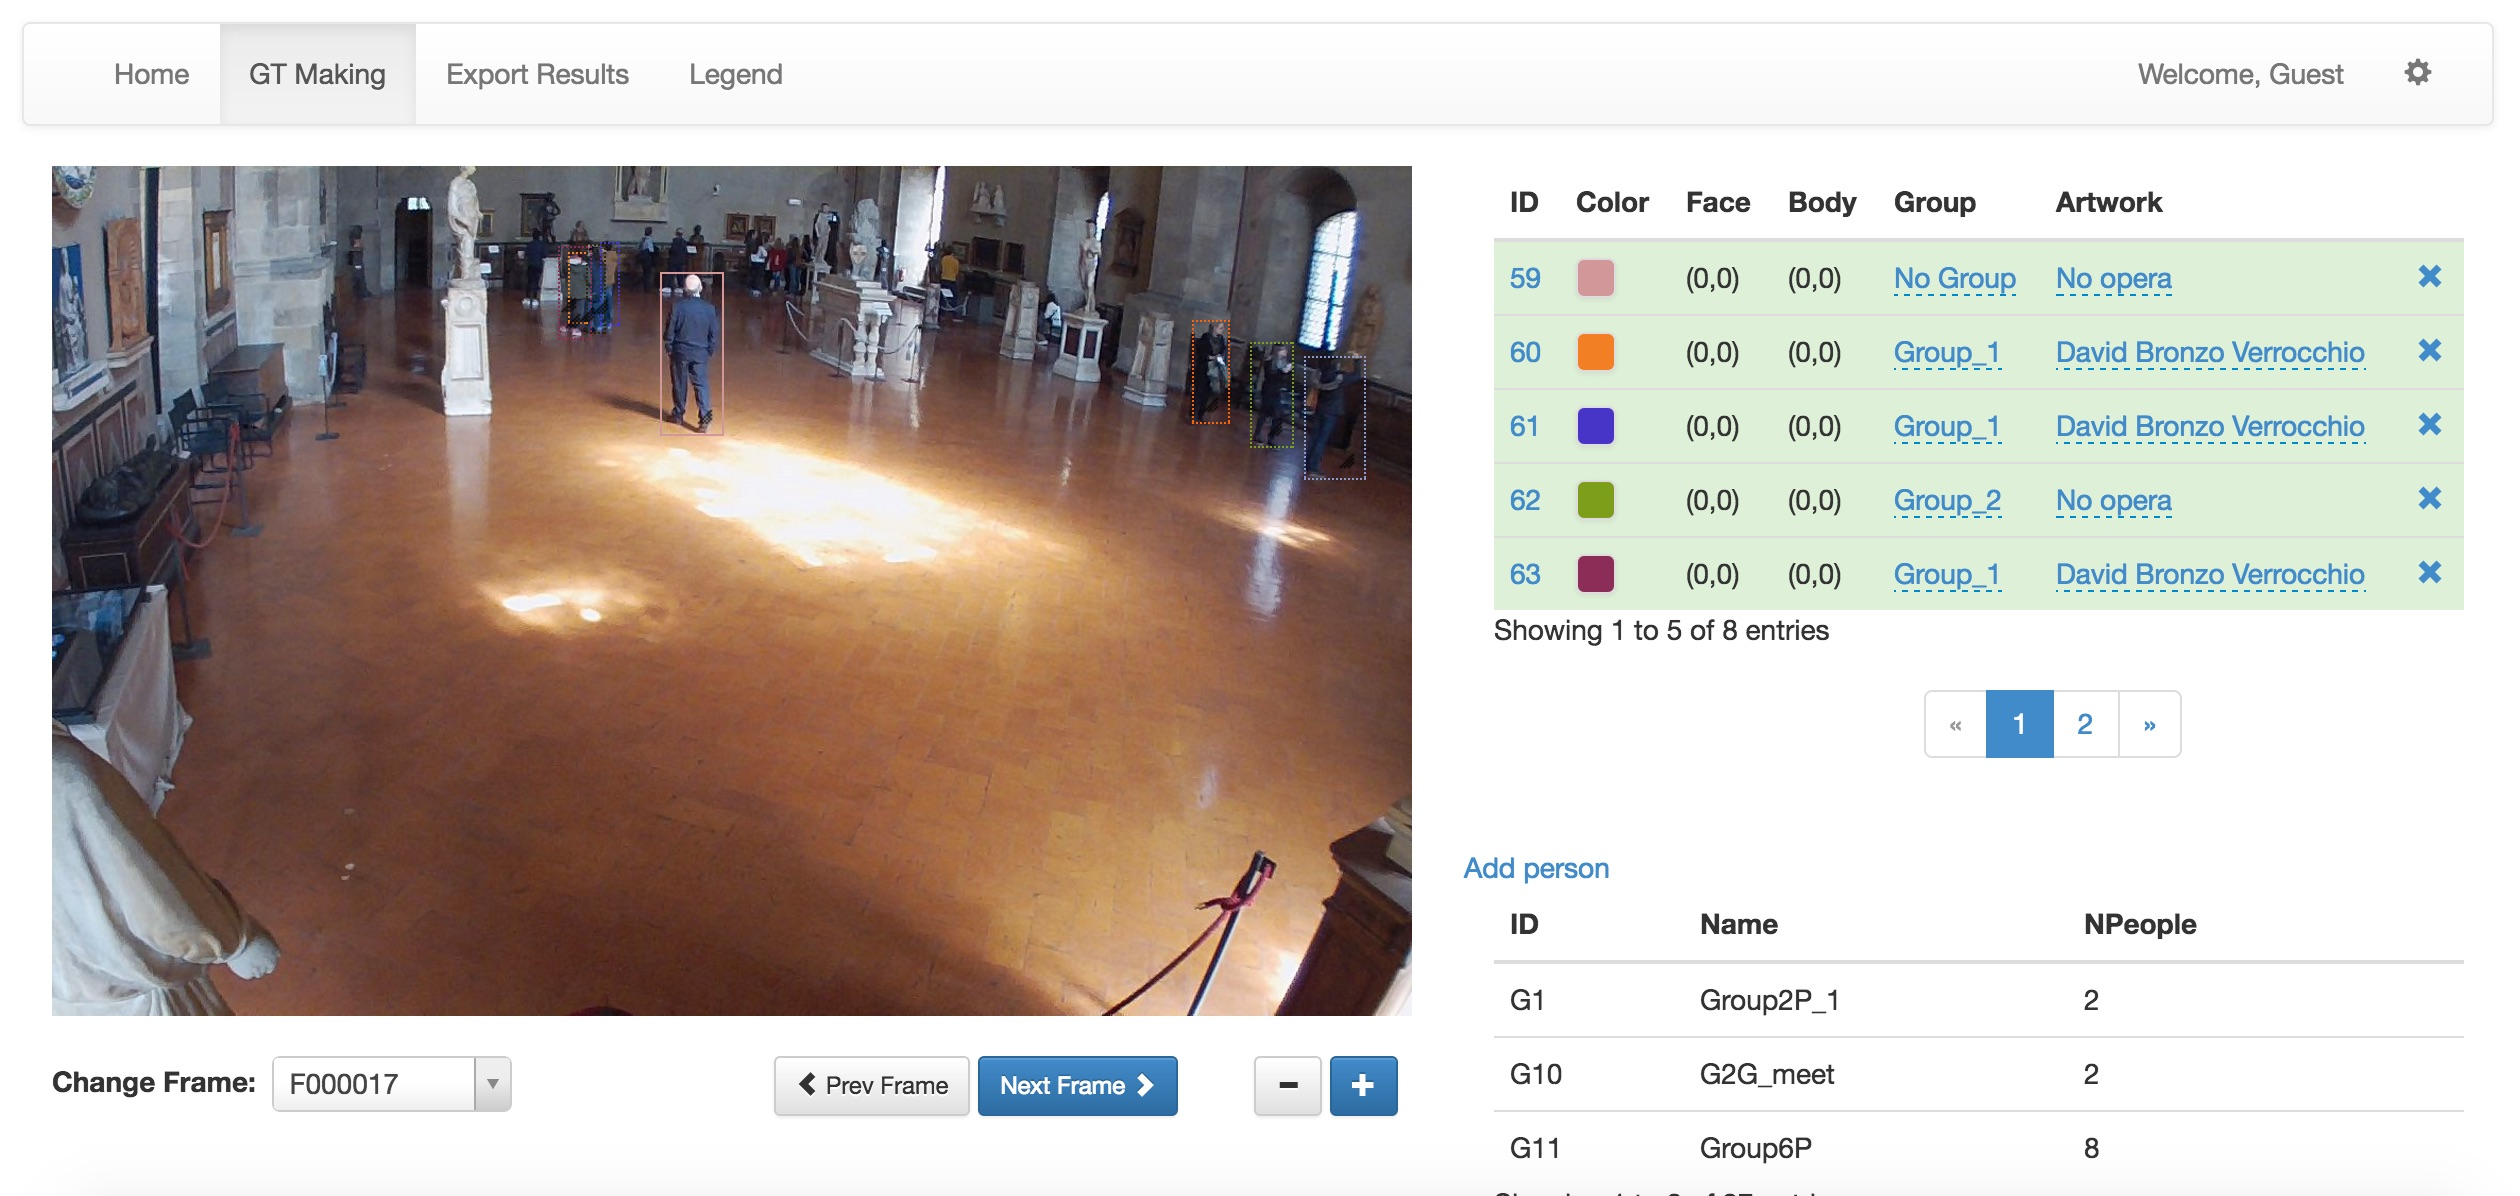
\includegraphics[width=1\textwidth]{images/watss_old.jpg}
\end{figure}
\end{tframe}

\begin{tframe}{User interface renovation}
The \textbf{new} WATSS user interface
\begin{figure}[h]
\centering
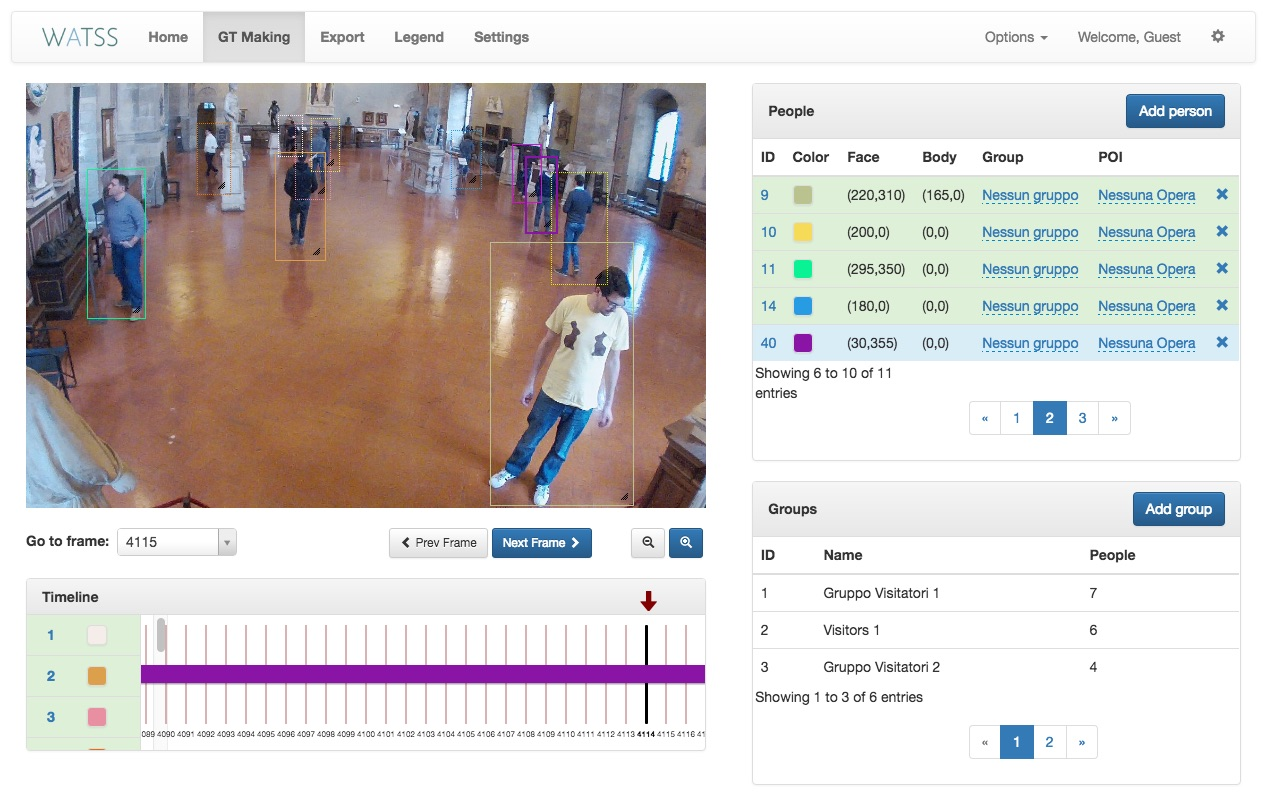
\includegraphics[scale=0.22]{images/watss-gui.jpg}
\end{figure}
\end{tframe}

\begin{tframe}{Video timeline}
In the video \textbf{timeline} all the video frames are shown, coloring the ones with at least one annotated person. 
\vspace{0.2cm}
\begin{figure}[h]
\centering
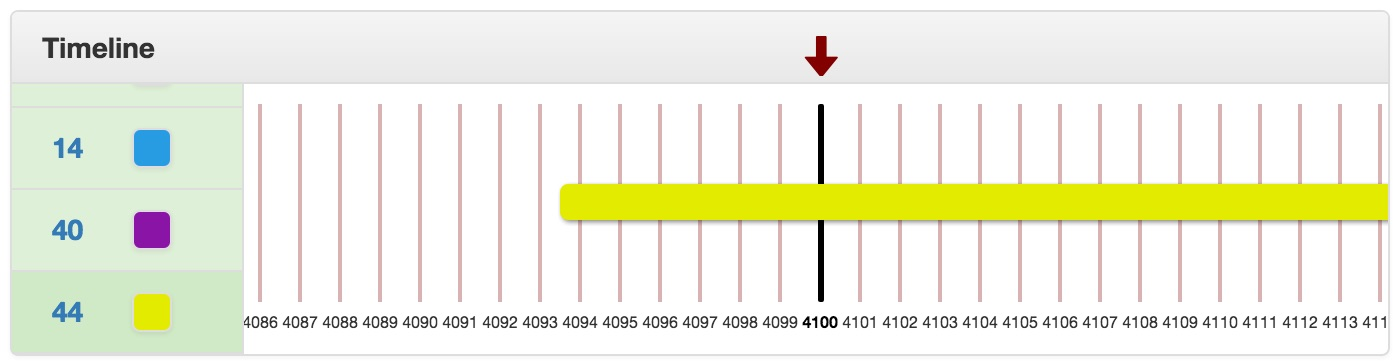
\includegraphics[scale=0.22]{images/timeline.jpg}
\end{figure}
\vspace{0.2cm}
Selecting a person in the list, the timeline displays its \textbf{history} highlighting frames where it is present. It is possible to navigate video frames by clicking on it.
\end{tframe}

\begin{tframe}{Proposals generation}
It is possible to generate \textbf{proposals} for a person in some selected frames based on previous  annotation of a it using timeline: just click and drag highlighted annotation.

\vspace{0.3cm}

Proposals generation is based on the combination of three different techniques:
\vspace{0.4cm}
\begin{itemize}
\item \textbf{Motion detection} using a \emph{background substractor}
\vspace{0.2cm}
\item \textbf{Pedestrian detection} using \emph{HOG descriptors}
\vspace{0.2cm}
\item \textbf{Kalman filter} for the \emph{motion estimation}
\end{itemize}
\end{tframe}


\begin{tframe}{Motion detection}
Motion detection is based on a \textbf{background substraction} method: moving objects are detected performing a subtraction between the current frame and a background model of the current scene, obtaining a \textbf{foreground mask}.

\vspace{0.3cm}
Each pixel of a frame is modeled as a \textbf{Mixture of Gaussians} and those which correspond to background colors are selected according to variance and persistence.

Pixel values that do not fit the background distributions are considered part of the foreground.

\vspace{0.2cm}
Background modeling consists of two main steps:
\begin{itemize}
\item \textbf{Background initialization}: background model evaluation.
\item \textbf{Background update}: background model is adapted to possible changes in the scene.
\end{itemize}
\end{tframe}


\begin{tframe}{Motion detection}
Using the foreground mask, a set of \textbf{detections} are extracted based on contours.
\begin{figure}[h]
\centering
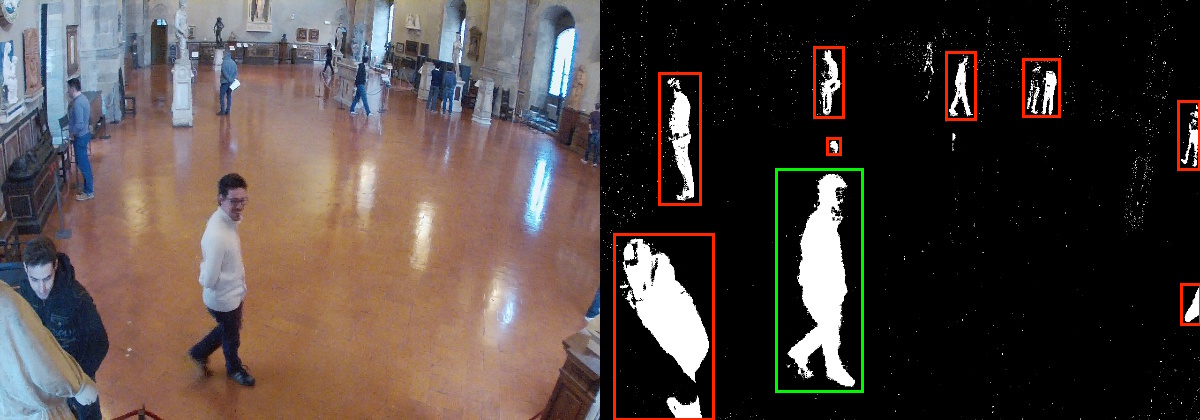
\includegraphics[width=1\textwidth]{images/frame_mog.jpg}
\end{figure}

Given the previous frame person bounding box, those that do not \emph{overlap} or are \emph{inconsistent} with its dimensions are discarded.
\end{tframe}

\begin{tframe}{Pedestrian detector}
The used \emph{pedestrian detection} technique is based on \textbf{Histogram of Oriented Gradients} and SVM classifier.

\begin{figure}[h]
\centering
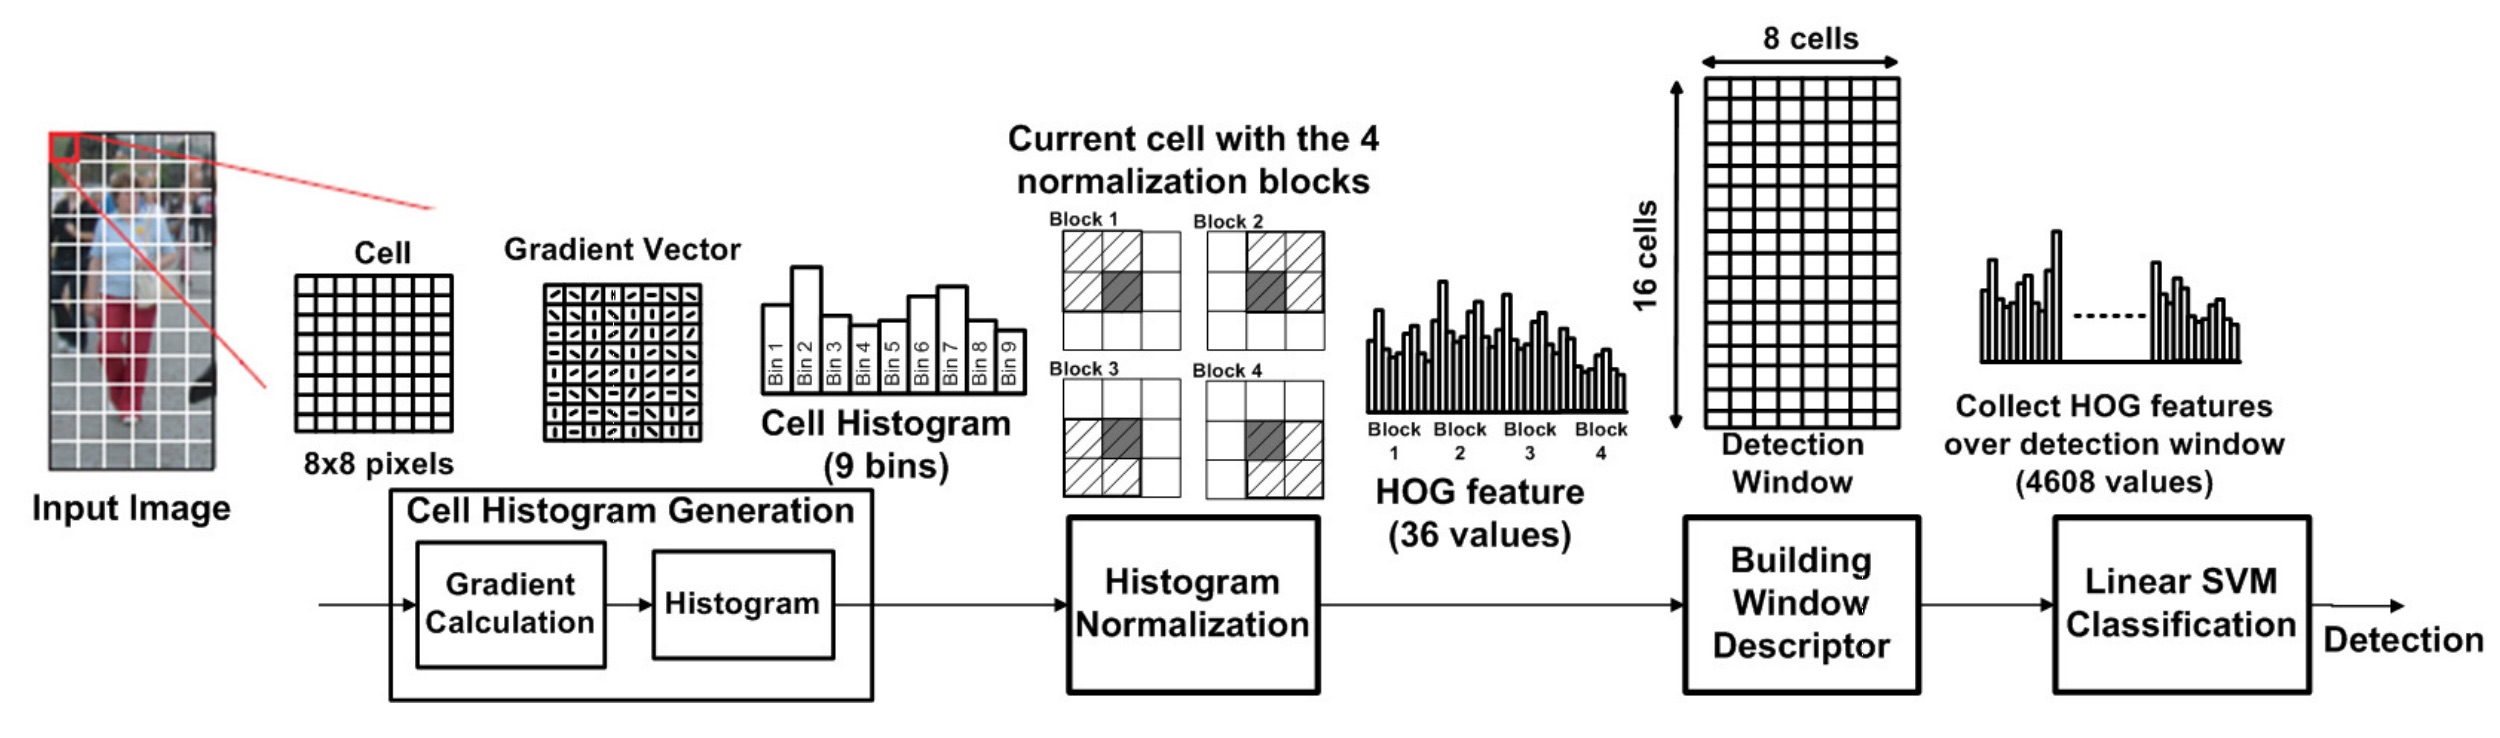
\includegraphics[width=1\textwidth]{images/hog_detector.jpg}
\end{figure}

As in the previous case, detections are filtered according to person history in scene.

\vspace{0.2cm}
\hfill {\tiny Figure from Suleiman, A., Sze, V. J Sign Process Syst (2016)}
\end{tframe}


\begin{tframe}{Kalman filter}

A \textbf{Kalman filter} is an optimal estimator used for following state estimation based on a set of previous observations.
\begin{figure}[h]
\centering
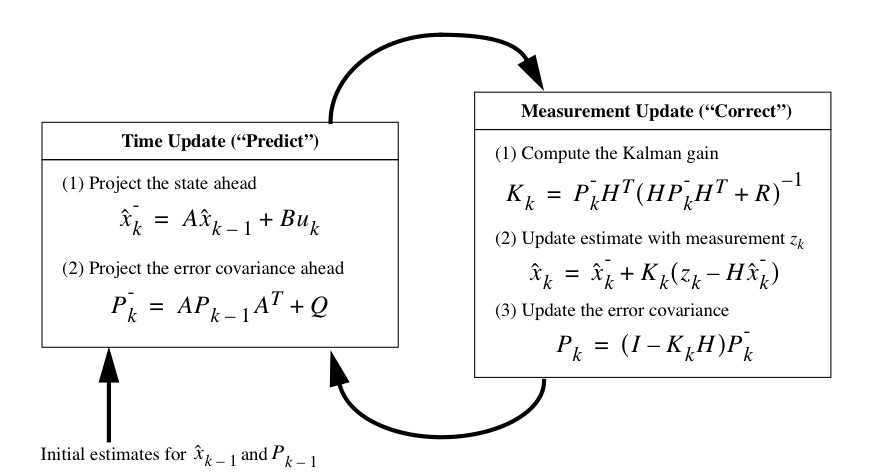
\includegraphics[width=0.6\textwidth]{images/kalmaneq.jpg}
\end{figure}
As system state is considered the \textbf{coordinates} $(x, y)$ \textbf{of the person} in the current scene, using motion and pedestrian detection for updating the measure.
\end{tframe}


\begin{tframe}{Proposals generation}
A proposal for a generic frame is the result of the combination of the above descripted methods. each resulted bounding box is compared with the previous frame annotation for evaluating a \textbf{score}:
\vspace{0.2cm}

$$score(r) = \frac{intersection(r, p)}{union(r, p)}$$

\vspace{0.3cm}

where $r$ is a resulting bounding box (\emph{i.e. the output of the motion detector}) and $p$ is the bounding box of the previous frame. 

\vspace{0.3cm}

If motion or pedestrian detector fails, then the \emph{Kalman filter prediction} is used as proposal.
\end{tframe}


\begin{tframe}{Proposals generation example}

\begin{figure}[h]
\centering
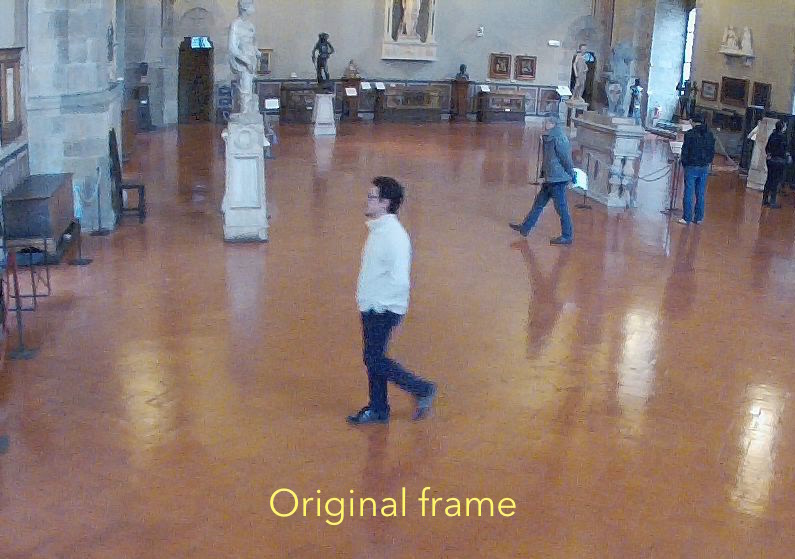
\includegraphics[width=.3\textwidth]{images/original.jpg}\quad
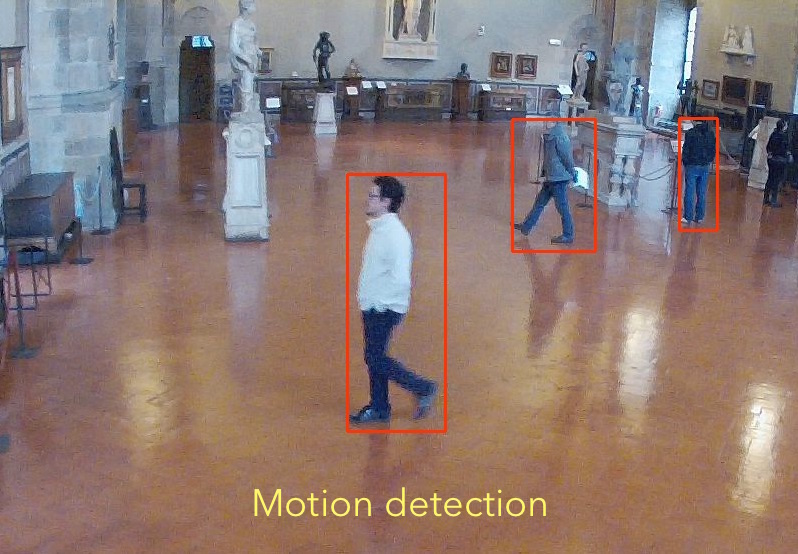
\includegraphics[width=.3\textwidth]{images/motion.jpg}\quad
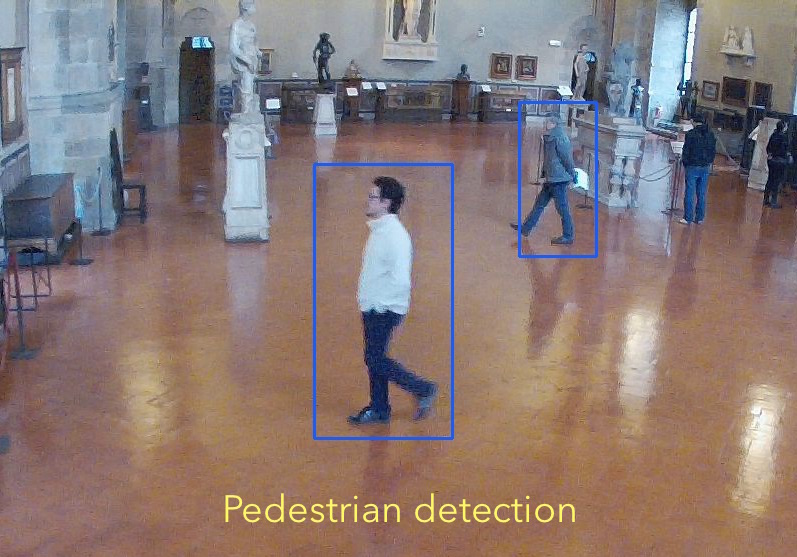
\includegraphics[width=.3\textwidth]{images/pedestrian.jpg}
\end{figure}

\begin{figure}[h]
\centering
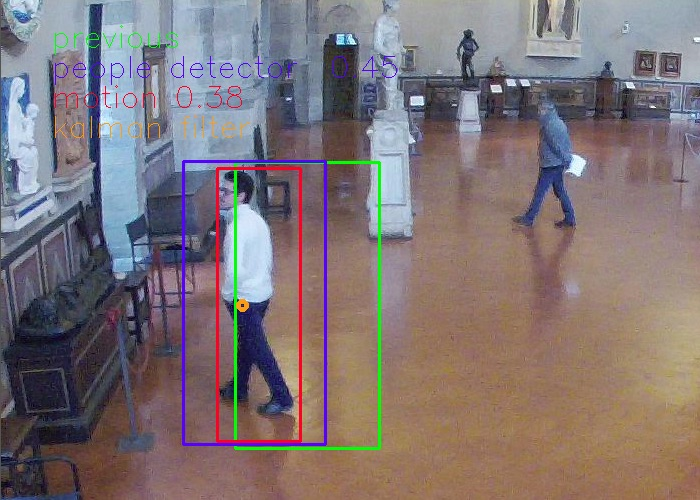
\includegraphics[width=.45\textwidth]{images/prediction1.jpg}\quad
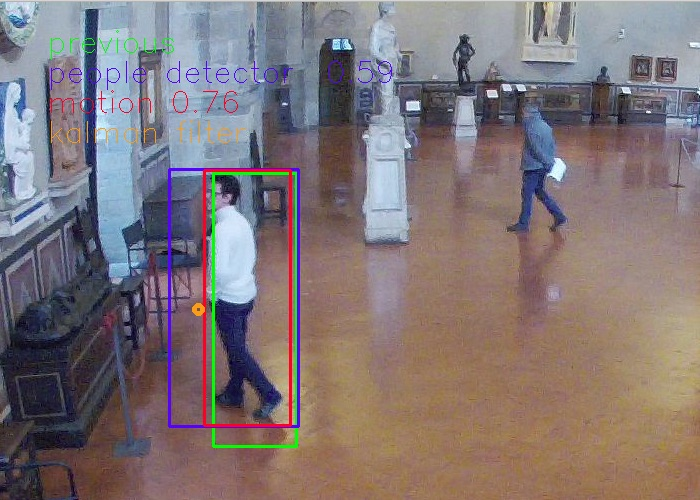
\includegraphics[width=.45\textwidth]{images/prediction2.jpg}\quad
\end{figure}

\end{tframe}


\begin{tframe}{Scene geometry}
In the annotation insertion step, it is possible to use\textbf{ scene geometry} knowledge in order to generate proposal based on the pointer position.

\vspace{0.5cm}
Requirements:
\vspace{0.3cm}
\begin{itemize}
\item \textbf{Static} cameras: they must be fixed in their positions
\vspace{0.2cm}
\item Camera \textbf{calibration parameters}
\vspace{0.2cm}
\begin{itemize}
\item \emph{Intrinsic} parameters, $\textbf{K}$
\item \emph{Estrinsic} parameters, rotation $\textbf{R}$ and translation $\textbf{t}$
\item A \emph{cross-ratio} \textbf{$\mu$}, being projective invariant
\end{itemize}
\end{itemize}
\end{tframe}

\begin{tframe}{Camera calibration}
Given $\textbf{X} = (X, Y, Z, 1)$, coordinates in \textbf{world}, and $\textbf{x} = (x, y, 1)$, coordinates in \textbf{scene}:
$$\textbf{x} = K [R | t] X$$
\begin{figure}[h]
\centering
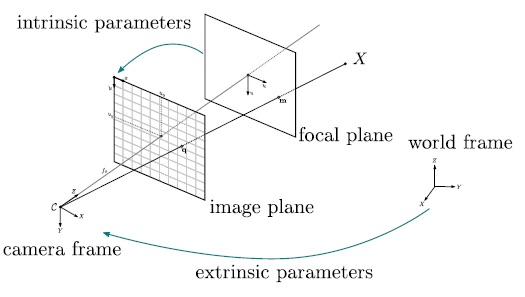
\includegraphics[width=0.8\textwidth]{images/camera.jpg}
\end{figure}
\end{tframe}

\begin{tframe}{Human height estimation}
From camera parameters, it is possible to evaluate \textbf{vanishing line} $\textbf{l}$ and \textbf{vanishing point} $\textbf{v}$


\begin{columns}[t] % align columns
\begin{column}{.45\textwidth}
$$l = P * [0, 0, 1]'$$
$$v = ((K')^{-1} * K^{-1}) * l$$
$$W = I + (\frac{1}{(1 - \mu)} - 1) * \frac{v * l'}{v' * l}$$

\vspace{0.2cm}
Giveng head position $head = (x, y, 1)$ and $\textbf{W}$:
$$feet = W^{-1} * head$$
$$height = |head_y - feet_y|$$

\end{column}%
\begin{column}{.5\textwidth}
\begin{figure}[h]
\centering
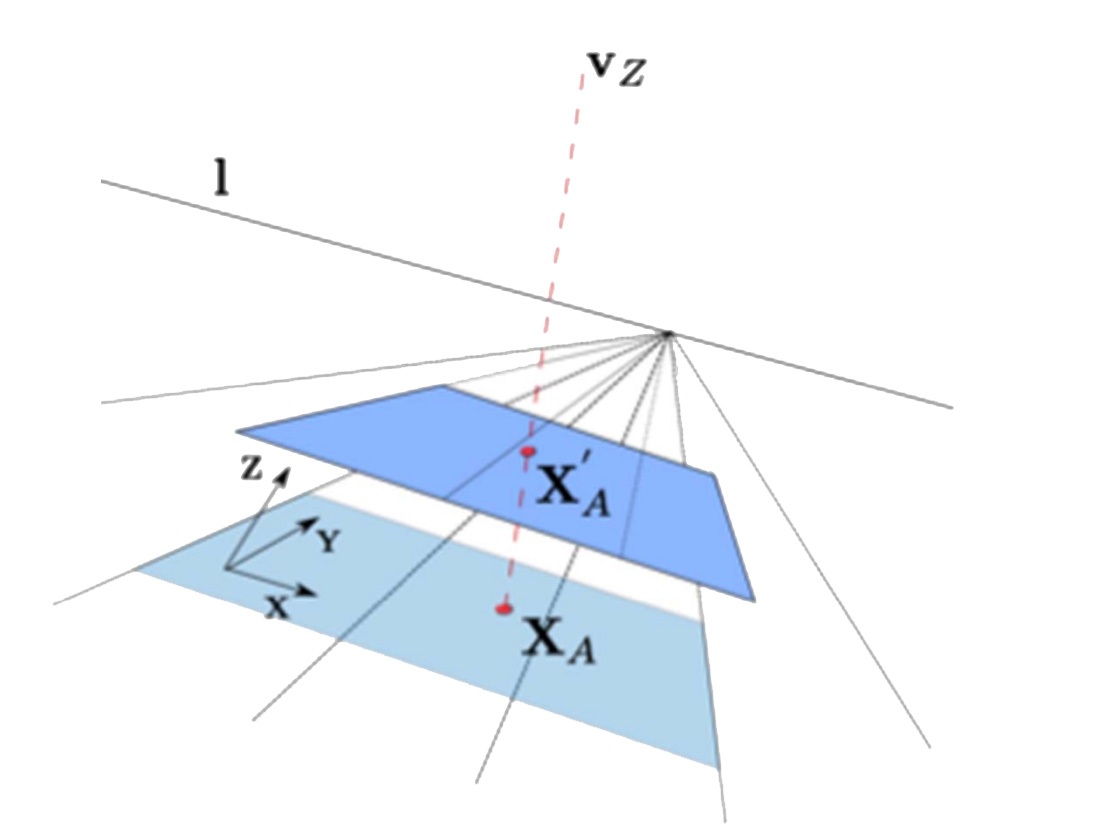
\includegraphics[width=1.1\textwidth]{images/height_calib.jpg}
\end{figure}
\end{column}%
\end{columns}


\end{tframe}


\begin{tframe}{References}

[1] O. M. Parkhi, A. Vevaldi, A. Zisserman, Deep Face Recognition, British Machine Vision Conference, 2015.

\vspace{0.1in}

[2] Davis E. King, Dlib-ml: A Machine Learning Toolkit, Journal of Machine Learning Research, 2009, 10, 1755-1758.

\vspace{0.1in}

[3] Chang, Chih-Chung and Lin, Chih-Jen, LIBSVM: A library for support vector machines, ACM Transactions on Intelligent System and Technology, 2, 3, 2011, 27:1—27:27.

\vspace{0.1in}

[4] A. Vevaldi and K. Lenc, MatConvNet: Convolutional Neural Networks for MATLAB, Proceedings of the ACM Int. Conf. On Multimedia, 2015.

\vspace{0.1in}

[5] A. Vevaldi and B. Fulkerson, VLFeat: An Open and Portable Library of Computer Vision Algorithms, 2008.


\end{tframe}

\end{document}